\chapter{21~cm observations: calibration, strategies, observables}
\label{chapter:bernardi}

\begin{bf}
  \author{Gianni Bernardi (INAF-IRA \& Rhodes University)}\\
  
Abstract\\

This chapter aims to provide a review of the basics of 21~cm interferometric observations and its methodologies. I begin by summarizing the main concepts of radio interferometry and their connection with the 21~cm observables - power spectra and images. I then provide a review of interferometric calibration and its interplay with foreground separation, including the current open challenges in calibration of 21~cm observations. I conclude with reviewing 21~cm instrument designs in the light of calibration choices and observing strategies.
\end{bf}


%\section{Chapter layout}
%\begin{itemize}
%\item review of basics of interferometry: van-Citter-Zernike theorem, $uv$-coverage, image formation;
%\item from visibilities to power spectra (in particular the delay transform approach - some overlap with Trott's chapter);
%\item interferometric calibration: impact on foreground subtraction, calibration errors redundant calibration;
%\item array design: power spectrum vs imaging, minimmum vs maximum redundancy - some overlap with Trott's chapter?;
%\item impact of calibration errors on power spectra;
%\item ionospheric impact/calibration;
%\item 21-cm image tomography;  
%\end{itemize}

\section{Interferometry overview}

\begin{figure}[]
\begin{center}
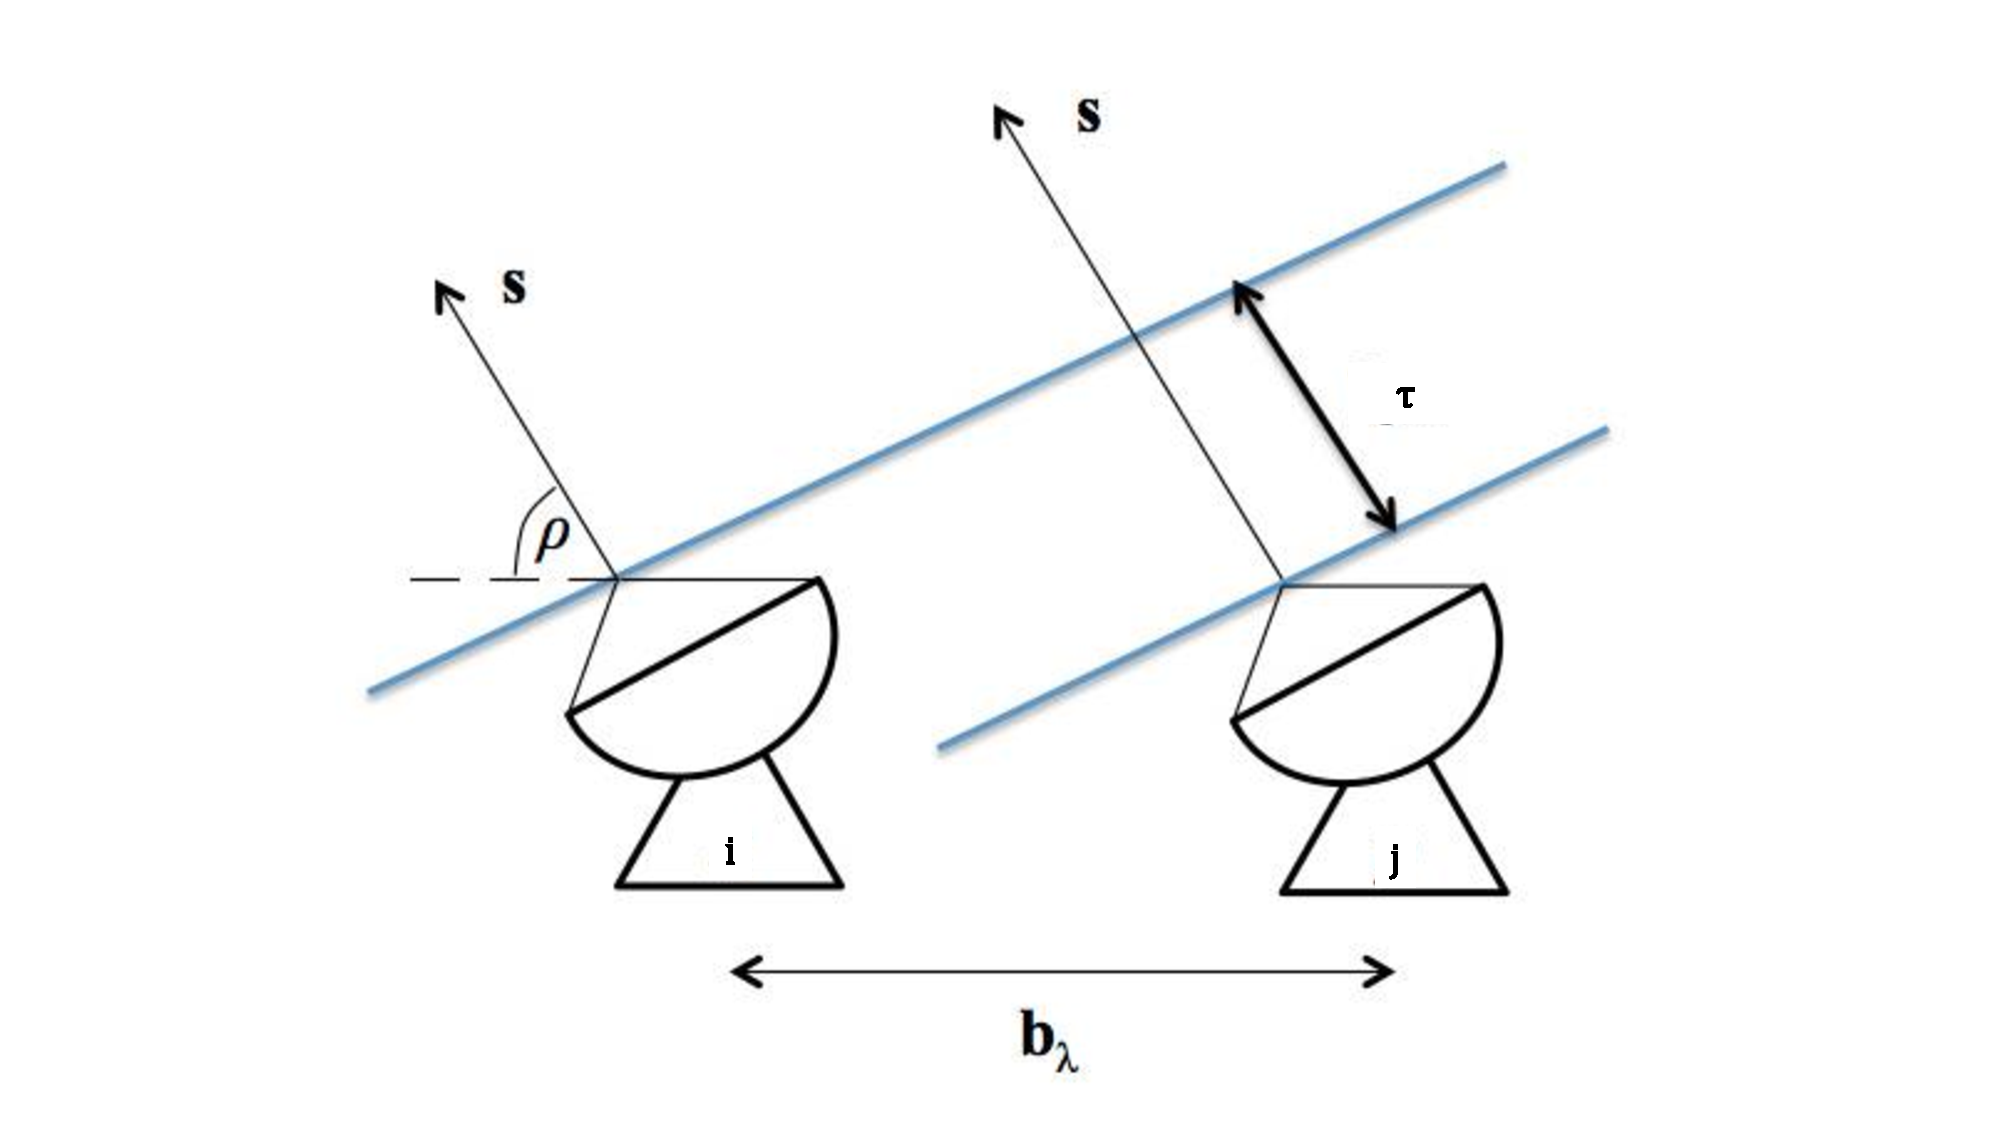
\includegraphics[width=1.\textwidth]{Bernardi/2_element_interferometer}
%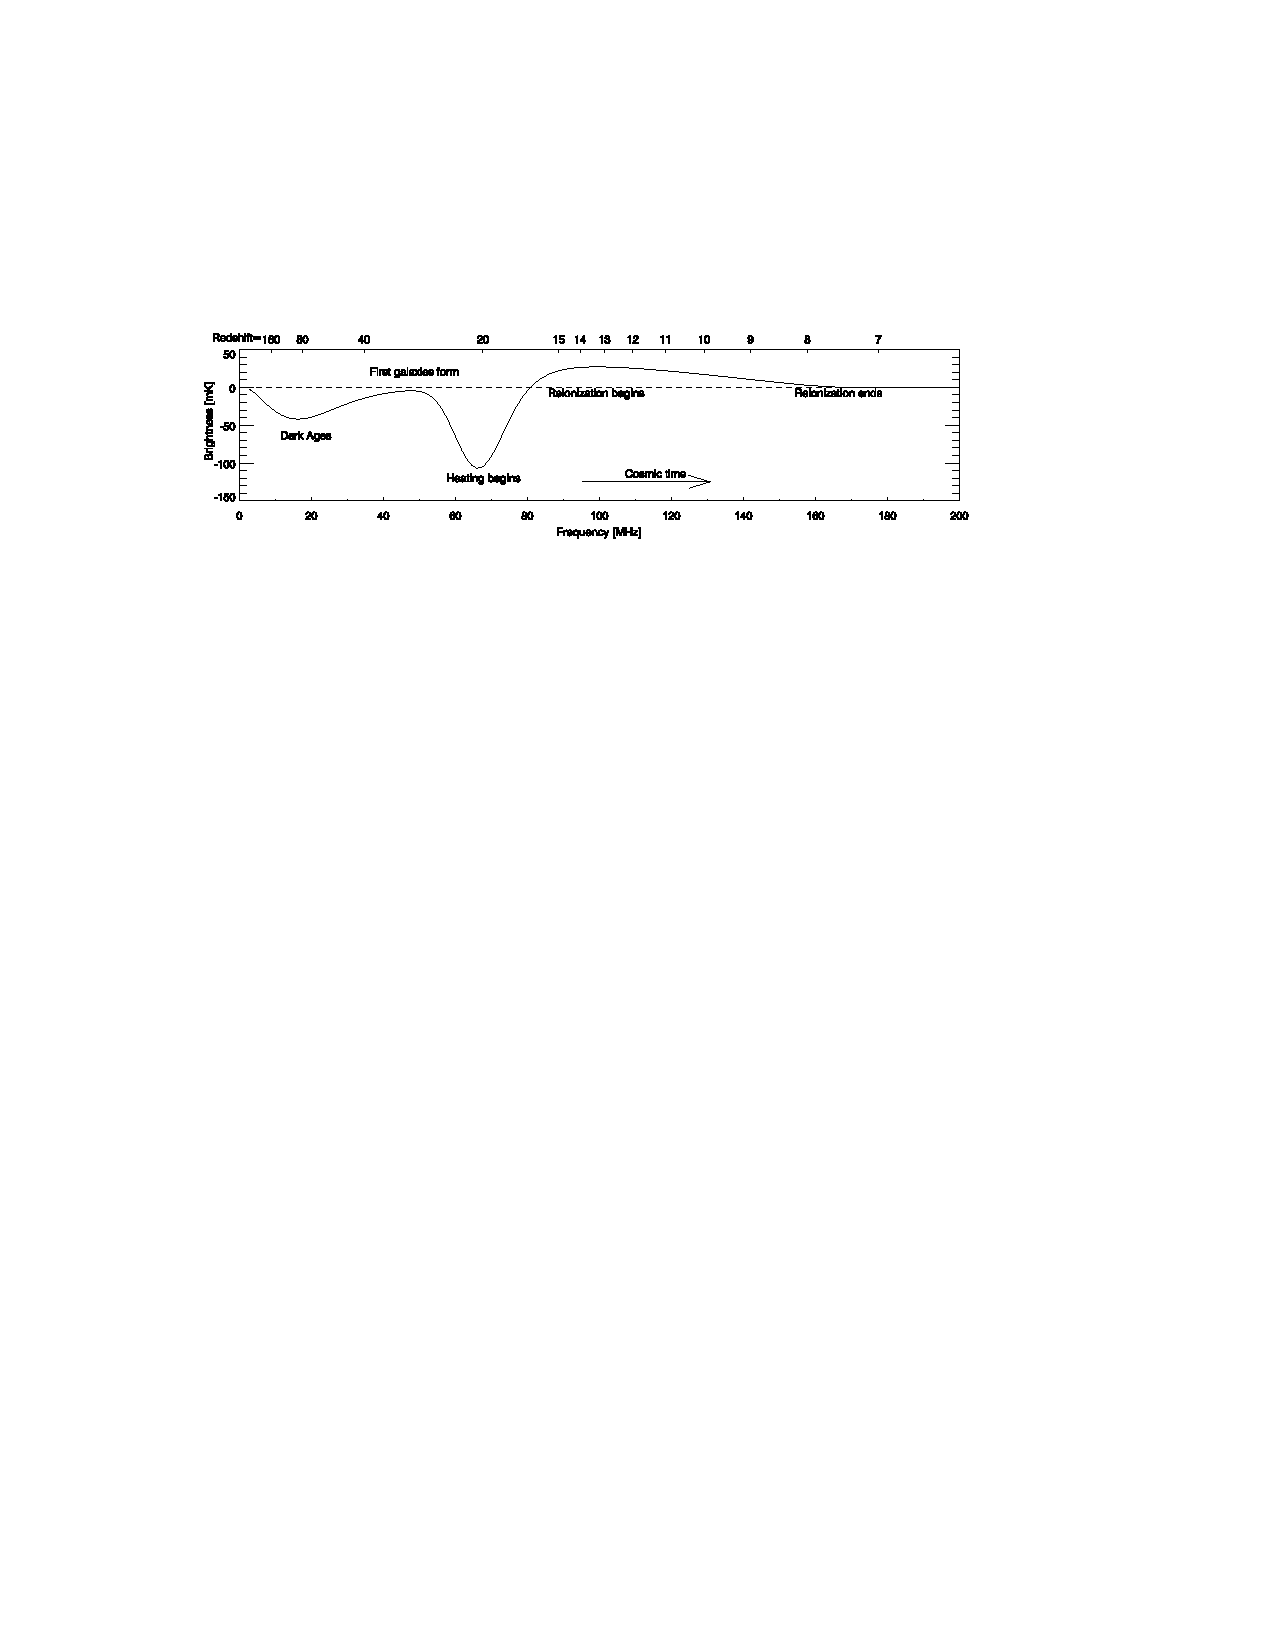
\includegraphics[trim = 0.2cm 0.6cm 0.2cm 0.2cm, scale = 1.0]{Greig/GlobalSignal}
\end{center}
%\caption{A standard schematic of the two element interferometer\footnote{Credit: http://inspirehep.net}.}
\caption{A standard schematic of the two element interferometer (from http://inspirehep.net).}
\label{fig:fig1}
\end{figure}

The Van Cittert-Zernike theorem expresses the fundamental relationship between the sky spatial brightness (or brightness distribution) $I$ and the quantity measured by an interferometer, i.e. the visibility $V$ (e.g., \cite{TMS}):
\begin{equation}
V_{ij} ({\bf b}, \lambda) = \int_\Omega {\bar I} (\hat{\sigma}, \lambda) \, e^{-2 \pi i {\bf b} \cdot {\hat \sigma}} d {\bf \sigma},
\label{eq:1}
\end{equation}
where ${\bf b}$ is the baseline vector that separates antenna~$i$ and antenna~$j$, and $\hat{sigma}$ is the observing direction (see Figure~\ref{fig:fig1}) and the integral is taken over the source size $\Omega$. The baseline vector is here specified in wavelengths, i.e. ${\bf b} = \frac{{\bf b_{\rm m}}}{\lambda}$, where ${\bf b_{\rm m}}$ is the baseline vector expressed in meters and $\lambda$ is the observing wavelength. It can be seen in Figure~\ref{fig:fig1}, that the celestial signal travels an extra path between the two antennas, and that length corresponds to a geometrical time delay $\tau = {\bf b} \cdot {\hat \sigma}$, where the word ``geometrical" refers to the fact that the delay depends upon the source position in the sky and the relative separation between the two antennas.

The sky brightness distribution does not enter directly in equation~\ref{eq:1}, but filtered by the antenna primary beam response $A$ that depends upon the direction in the sky and the wavelength, i.e. ${\bar I} ({\bf b}, \lambda) = A ({\bf b}, \lambda)  \, I ({\bf b}, \lambda)$. The response of the primary beam attenuates the sky emission away from the pointing direction, effectively reducing the field of view $\theta$ of the instrument. Generally speaking, the size of the field of view is essentially given by the antenna diameter $D$: 
\begin{equation}
\theta \approx \frac{\lambda}{D}.
\label{eq:2}
\end{equation}
Equation~\ref{eq:1} is often re-written in a different coordinate system, i.e. using the components of the baseline vector $(u,v,w)$ and the reciprocal $(l,m,n)$, where $(l,m)$ are the coordinates in the plane on the sky tangent to the observing direction $n$ (for a detailed discussion of coordinate systems see, for example \cite{TMS}). Using this coordinate system, equation~\ref{eq:1} becomes (e.g., \cite{TMS}):
\begin{equation}
V_{ij} (u,v,w, \lambda) = \int_\Omega {\bar I} (l, m, \lambda) \, e^{-2 \pi i (ul + vm + w(n - 1))} \frac {dl \, dm \, dn}{\sqrt{1 - l^2 - m^2}},
\label{eq:3}
\end{equation}
Although low frequency radio observations are intrinsically wide-field, for the purpose of studying the 21~cm observables, we can reduce equation~\ref{eq:3} to a two dimensional Fourier transform:
\begin{equation}
V_{ij} (u,v, \lambda) = \int_\Omega {\bar I} (l, m, \lambda) \, e^{-2 \pi i (ul + vm)} dl \, dm.
\label{eq:4}
\end{equation}
Equation~\ref{eq:4} indicates that an {\it interferometer measures the two dimensional Fourier transform of the spatial sky brightness distribution}. If our goal is to reconstruct the sky brightness distribution, equation~\ref{eq:4} can be inverted into its corresponding Fourier pair:
\begin{equation}
%{\bar I} (l, m, \lambda) = \int_{- \infty}^{+ \infty} V_{ij} (u,v, \lambda) \, e^{2 \pi i (ul + vm)} du \, dv.
{\bar I} (l, m, \lambda) = \int V_{ij} (u,v, \lambda) \, e^{2 \pi i (ul + vm)} du \, dv.
\label{eq:5}
\end{equation}
Equation~\ref{eq:5} is, however, a poor reconstruction of the sky brightness distribution as only one Fourier mode is sampled at a single time instance. Strictly speaking, indeed, all the quantities in equation~\ref{eq:4} and \ref{eq:5} are time variable. In most cases, the time dependence of the primary beam and the sky brightness distribution can be neglected, however, this is not the case for the visibility $V$ as the projection of the baseline vector with respect to the source direction changes significantly throughout a long (e.g. a few hours) track. In this way, many measurements of the visibility coherence function $V$ can be made as $(u,v)$ change with time, allowing for a better reconstruction of the ${\bar I} (l, m, \lambda)$ function. This methods is commonly referred to as {\it filling the $uv$ plane via Earth rotation synthesis} and was invented by \cite{ryle60}. The other (complementary) way to fill the $uv$ plane is to deploy more antennas on the ground in order to increase the number of instantaneous measurements of independent Fourier modes. If $N$ antennas are connected in an interferometric array, $\frac{N (N - 1)}{2}$ instantaneous measurements are made. 

The combination of a large number of antennas and the Earth rotation synthesis, defines the sampling function $S(u,v)$ in the $uv$ plane. In any real case, equation~\ref{eq:5} can therefore be re-written as:
\begin{equation}
{\bar I}_D (l, m, \lambda) = \int S(u,v, \lambda) V (u,v, \lambda) \, e^{2 \pi i (ul + vm)} du \, dv,
\label{eq:6}
\end{equation}
where ${\bar I}_D$ indicates the sky brightness distribution sampled at a finite number of $(u,v)$ points (often termed {\it dirty image}) and where the explicit dependence on the antenna pair was dropped for simplicity. Using the convolution theorem, equation~\ref{eq:6} can be re-written as:
\begin{equation}
{\bar I}_D (l, m, \lambda)  =  \tilde{S \, V} =  {\tilde S} \ast {\tilde V} = {\rm PSF} (l, m, \lambda) \ast {\tilde V} (l, m, \lambda),
\label{eq:7}
\end{equation}
where the tilde indicates the Fourier transform, $\ast$ the convolution operation and PSF is the Point Spread Function, i.e. the response of the interferometric array to a point sources which, in our case, is also the Fourier transform of the $uv$ coverage.

%I will give some examples of sampling functions for different instruments in Section~\ref{sec:design}, however, 
The sampling function always effectively reduces the integral over a finite (often not contiguous) area of the $uv$ plane. In particular, the sampled $uv$ plane is restricted to a minimum $uv$ distance that cannot be shorter than the antenna\footnote{In this chapter I use the words ``antenna" and ``station" interchangeably to indicate the correlated elements even if, in the literature, they are normally used to indicate a dish and and a dipole, or a cluster of dipoles, respectively.} size and the largest separation between antennas, i.e. the maximum baseline ${\bf b}_{\rm max}$. The maximum baseline also sets the maximum angular resolution $\theta_b$:
\begin{equation}
\theta_b \approx \frac{\lambda}{|{\bf b}_{\rm max}|}.
\label{eq:8}
\end{equation}
The incomplete sampling of the $uv$ space leads to a PSF that has ``sidelobes", i.e. nulls and secondary lobes that can often contaminate fainter true sky emission. The best reconstruction of the sky brightness distribution ${\bar I}$ requires deconvolution of the dirty image from the PSF. 




\section{21~cm observables: power spectra and images}
\label{sec:observables}

The ultimate goal of 21~cm observations is to image the spatial distribution of the 21~cm signal as a function of redshift, also known as {\it 21~cm tomography}. Given the curent theoretical predictions, such observations need to achieve mK sensitivity on a few arcminute angular scales (see Chapter~1 in this book). Most of the current arrays, however, only have the sensitivity to perform a statistical detection of the 21~cm signal, i.e. to measure its power spectrum. Given an intensity field $T$, function of the three dimensional spatial coordinate $\bf x$, its power spectrum $P(k)$ is defined as:
\begin{equation}
%\langle {\tilde T}^* ({\bf k}) {\tilde T}({\bf k'}) \rangle = (2 \pi)^3 P({\bf k}) \delta^3({\bf k} - {\bf k}')
\langle {\tilde T}^* ({\bf k}) {\tilde T}({\bf k'}) \rangle = (2 \pi)^3 P(k) \delta^3({\bf k} - {\bf k}')
\label{sec_observables_eq1}
\end{equation}
where $\langle \rangle$ indicates the ensamble average, $\bf k$ is the Fourier conjugate of $\bf x$, tilde the Fourier transform, $^*$ the conjugate operator and $\delta$ the Dirac delta function. In 21~cm observations, power spectra can be computed directly from interferometric image cubes after deconvolution of the dirty image ${\bar I}_D (l,m,\lambda)$ from the point spread function (e.g., \cite{pen09}, \cite{harker10}, \cite{beardsley16}, \cite{patil17}). Alternatively, the 21~cm power spectrum can be estimated directly from the interferometric visibilities. Equation~\ref{eq:4} already shows that the interferometer is a ``natural" spatial power spectrum instrument (e.g., \cite{white99}). Visibilities can be further Fourier transformed along the frequency axis (the so-called {\it delay trasform}, \cite{parsons12a}): 
\begin{equation}
{\tilde V}_{ij} (u,v, \tau) = \int_B {\bar I} (l, m, \nu) \, e^{-2 \pi i \nu \tau} d \nu
\label{sec_observables_eq2}
\end{equation}
where $B$ is the observing bandwidth and $\tau$ is the geometrical delay. The delay transform is therefore proportional to the three dimensional power spectrum (\cite{parsons12b}):
\begin{equation}
P(k) \propto {\tilde V}_{ij} (|{\bf b}|, \tau),
\label{sec_observables_eq3}
\end{equation}
where the proportionality constant transforms the visibility units into power units (\cite{parsons12b}). The observer units $({\bf b},\tau)$ map directly in $k$ modes parallel and perpendicular to the line of sight (e.g., \cite{morales04}):
\begin{equation}
k_\perp = \frac{2 \pi |{\bf b}|}{D_c} = \frac{2 \pi \sqrt{u^2 + v^2}}{D_c}, \,\,\,\,\,\,\,    k_\parallel = \frac{2 \pi f_{21} H_0 E(z)}{c \, (1 + z)^2} \, \tau,
\label{sec_observables_eq4}
\end{equation}
where $D_c$ is the transverse comoving distance, $f_{21} = 1421$~MHz, $H_0$ is the Hubble constant and $E(z) = \sqrt{\Omega)m (1+z)^3 + \Omega_k (1+z)^2 + \Omega_\Lambda}$. Due to the dependence of the geometrical delay upon frequency, equation~\ref{sec_observables_eq3} is only valid for short baselines, typically shorter than a few hundresd meters, for which the geometrical delay is fairly constant across the bandwidth and lines of constant $k_\parallel$ are essentially orthogonal to the $k_\perp$ axis (\cite{parsons12b}).

Equation~\ref{sec_observables_eq2} does not only provide a link between visibilities and three dimensional power spectra, but also introduces the concept of ``horizon limit", i.e. the maximum physical delay allowed $\tau_{\rm max} = \frac{|{\bf b}|}{c}$, where $c$ is the speed of light. The most relevant implication of the existence of an horizon limit is the definition of a region in the two dimensional $(k_\parallel,k_\perp)$ power spectrum space where smooth-spectrum foregrounds are confined, leaving the remaining area  uncontaminated in order to measure the 21~cm signal (the so-called ``Epoch of Reionization (EoR) window", Figure~\ref{fig:fig2}). Foregrounds can therefore be ``avoided" with no requirements for subtraction (e.g., \cite{morales12}, \cite{vedantham12}, \cite{pober13}, \cite{thyagarajan13}; see also Chapter~6 in this book).
\begin{figure}[]
\begin{center}
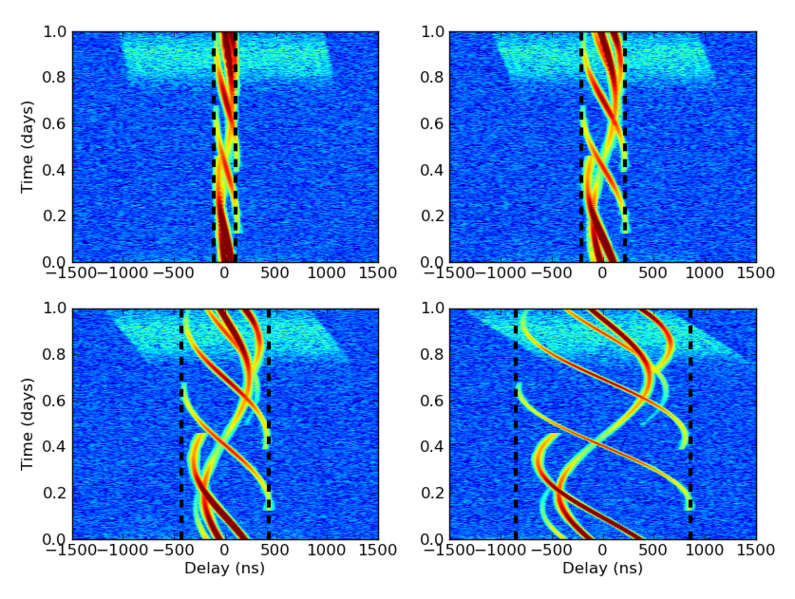
\includegraphics[width=1.\textwidth]{Bernardi/delay_transform}
\end{center}
\caption{Amplitude of delay transformed visibilities as a function of time and delay for a 32 (top let), 64 (top right), 128 (bottom left) and 256~m (bottom right) baselines respectively (from \cite{parsons12a}). A number of smooth spectrum point sources are simulated as foregrounds and their tracks are clearly bound within the horizon limit (black dashed line). The cyan emission is a fiducial 21~cm model that has power up to high delays regardless of the baseline length.}
\label{fig:fig2}
\end{figure}
The choice of a foreground avoidance strategy versus subtraction plays an important role in planning an experiment, its related observing strategy and the array calibration strategy.

The requirements for image tomography are the same as for high brightness sensitivity observations of diffuse emission like the Cosmic Microwave Background (e.g., \cite{halverson02}, \cite{dickinson04}, \cite{readhead04}). The 21~cm spatial distribution throughout cosmic reionization has structures on 5-10 arcminutes up to degree scales (e.g., \cite{majumdar12}, \cite{datta12}, \cite{mellema13}, \cite{kakiichi17}). In order to image 21~cm fluctuations, a maximum baseline of the order of a few km gives a resolution of a few arcminutes in the $100-200$~MHz range, together with filled $uv$ plane in order to accurately reconstruct their complex spatial structure. A filled $uv$ plane also leads to a PSF with very low sidelobes, making the deconvolution process easier. The most stringent requirements for image tomography remain the accurate foregrond separation and, as I will review in the next section, the related instrumental calibration.



%\section{Challenges in 21~cm observations: interferometric calibration in presence of bright foreground emission, wide fields of view, ionosphere}
\section{Interferometric calibration and 21~cm observations}
\label{sec:challenges}

Celestial radio signals always experience a corruption when observed with an interferometric array, due to the non-ideal instrumental response that is corrected in post processing in a process that is known as interferometric calibration. Calibration relies on the definition of a data model where the corruptions are described by antenna based quantities known as Jones matrices. Such data model is known as the interferometric measurement equation (\cite{hamaker96},\cite{smirnov11},\cite{smirnov11b},\cite{smirnov11c}).

If antenna $1$ and antenna $2$ measure two orthogonal, linear polarizations $x$ and $y$, the cross-polarization visibility products can be grouped in a $2 \times 2$ complex matrix ${\bf V}$:
\begin{equation}
    {\bf V}_{12} (u,v,\lambda) \equiv 
    \left[ 
    \begin{array}{cc}
    V_{12,xx} (u,v,\lambda) & V_{12,xy} (u,v,\lambda) \\
    V_{12,yx} (u,v,\lambda) & V_{12,yy} (u,v,\lambda) \\
    \end{array}
    \right].   
\label{eq:sec:1}
\end{equation} 
The sky brightness distribution $I$ can also be written as a $2 \times 2$ matrix ${\bf B}$ using the Stokes parameters as a polarization basis:
\begin{equation}
    {\bf B}_I (l,m,\lambda) \equiv 
    \left[
    \begin{array}{cc}
    I (l,m,\lambda) + Q (l,m,\lambda) & U (l,m,\lambda) + iV (l,m,\lambda) \\
    U (l,m,\lambda) - iV (l,m,\lambda) & I (l,m,\lambda) - Q (l,m,\lambda) \\
    \end{array}
    \right].   
\label{eq:sec:2}
\end{equation} 
At this point, equation~\ref{eq:3} can be written by including the corruptions represented by the complex Jones matrices $J$: (\cite{hamaker96},\cite{smirnov11}):
\begin{equation}
{\bf V}_{12} (u,v,\lambda) = {\bf J}_1 \left( \int_\Omega {\bf B}_I (l, m, \lambda) \, e^{-2 \pi i (ul + vm)} dl \, dm  \right) {\bf J}_2^H
\label{eq:sec:3}
\end{equation} 
Equation~\ref{eq:sec:3} is known as the {\it measurement equation} and is the core of interferometric calibration. For an array with $N$ antennas, equation~\ref{eq:sec:3} can be written for each of the $\frac{N (N - 1)}{2}$ visibilities forming an overdetermined system of equations. The development of  algorithms to solve the calibration system of equations is a very active research line (\cite{mitchell08}, \cite{kazemi11}, \cite{tasse14}, \cite{yatawatta15}, \cite{smirnov15}) although beyond the scope of this chapter and we mention it here for completeness.

The solution of the measurement equation requires some knowledge of the sky brightness distribution ${\bf B}_I$, in other words, a {\it sky model}. Traditionally this is achieved by observing a calibration source, i.e. a bright, unresolved point source with known spectral and polarization properties. Calibration solutions are then applied to the observed field that is then used to improve the sky model ${\bf B}_I$ which, in turn, leads to more accurate calibration solutions ${\bf J}$. This loop is traditionally called self calibration (\cite{cornwell81}, \cite{pearson84}) and can lead to a highly accurate calibration (e.g., \cite{bernardi10}, \cite{smirnov11b}).

The advantage of the measurement equation is that it can factorize different physical terms into different matrices. For example, the frequency response of the telescope electronics and its time variations essentially affects only the two polarization response and are modeled with a diagonal Jones matrix ${\bf B}$:
\begin{equation}
    {\bf B} (t,\lambda) \equiv 
    \left[
    \begin{array}{cc}
    b_x (t,\lambda) 	& 	0 	\\
    0 		& b_y (t,\lambda) 	\\
    \end{array}
    \right],   
\label{eq:sec:4}
\end{equation} 
where we made it explicit that ${\bf B}$ can vary with time and frequency. The undesired instrumental leakage between the two orthogonal polarized can be written as a ${\bf D}$ Jones matrix of the form:
\begin{equation}
    {\bf D} (t,\lambda) \equiv 
    \left[
    \begin{array}{cc}
    1	 		& d_x (t,\lambda)	\\
    -d_y (t,\nu)	& 1 	\\
    \end{array}
    \right],   
\label{eq:sec:5}
\end{equation} 
and the measurement equation can be written as:
\begin{equation}
{\bf V}_{12} (u,v,\lambda) = {\bf B}_1 \, {\bf D}_1 \left( \int_\Omega {\bf B}_I (l, m, \lambda) \, e^{-2 \pi i (ul + vm)} dl \, dm  \right) {\bf D}_2^H  \, {\bf B}_2^H.
\label{eq:sec:6}
\end{equation}
We note that, in principle, the primary beam response should appear as an additional $2 \times 2$ Jones matrix before the ${\bf D}$ matrix. For the purpose of this section we will neglect it, although we will illustrate an exception to this assumption when we later discuss about polarization calibration.

Retaining only the first order terms, equation~\ref{eq:sec:6} can be written as (\cite{sault96}):
\begin{eqnarray}
V_{12,xx} (u,v,\lambda) & = & b_{1,x} \, b_{2,x}^* [V_I (u,v,\lambda) - V_Q (u,v,\lambda)]\\
V_{12,xy} (u,v,\lambda) & = & b_{1,x} \, b_{2,y}^* [(d_{1,x} - d_{2,y}^*) V_I (u,v,\lambda) + V_U (u,v,\lambda) + iV_V (u,v,\lambda)]	\\
V_{12,yx} (u,v,\lambda) & = & b_{1,y} \, b_{2,x}^* [(d_{2,x} - d_{1,y}^*) V_I (u,v,\lambda) + V_U (u,v,\lambda) - iV_V (u,v,\lambda)]	\\
V_{12,yy} (u,v,\lambda) & = & b_{1,y} \, b_{2,y}^* [V_I (u,v,\lambda) - V_Q (u,v,\lambda)],
\label{eq:sec:7}
\end{eqnarray}
where we dropped the explicit dependence on time and wavelength from the Jones matrices for notation clarity and where $V_{i=I, Q, U, V}$ are the Fourier transforms of the elements of the sky brightness matrix ${\bf B}$.

This form of the measurement equation offers an intuitive understanding as to why calibration is of paramount important in 21~cm observations. The observed visibilities are essentially a measurement of foreground emission and, in the ideal case, their amplitudes would vary smoothly with frequency, allowing to avoid or subtract foregrounds. However, the instrumental response inevitably corrupts this smoothness in several ways: because the telescope primary beam is not sufficiently smooth in frequency, because of the electronic response or because of reflections along the signal path. Although calibration will correct for these effects and restore the intrinsic foreground frequency smoothness, calibration errors (i.e., deviations from the true ${\bf B}$ solutions) will still corrupt the foreground spectra. In practice, calibration errors result into foreground power leaking out of the horizon limit and jeopardizing (part of) the EoR window. The corruption of the foreground spectra will limit the accuracy of any subtraction method (see discussion in Chapter~6 in this book). {\it The effectiveness of foreground separation, proven in ideal cases, depends significantly on the accuracy of interferometric calibration.}

The form of the measurement equation written in equations~\ref{eq:sec:6} and \ref{eq:sec:7} is often referred to as a {\it direction independent} calibration as it implicitly assumes that a single Jones matrix is sufficient to describe corruptions across the whole sky area of interest. This assumption is often invalid at low frequencies, mostly because of the changing primary beam response over a wide field of view, frequency, and the course of the observation, and the position and time dependent corruptions introduced by the Earth's ionosphere. In this case the measurement equation becomes {\it direction dependent}, i.e. a different Jones matrix is written and solved for a certain number of directions in the sky:
\begin{equation}
{\bf V}_{12} (u,v,\lambda) = \sum_s \left[ {\bf B}_{1,s} \left( \int_\Omega {\bf B}_{I,s} (l, m, \lambda) \, e^{-2 \pi i (ul + vm)} dl \, dm  \right) {\bf B}_{2,s}^H \right],
\label{eq:sec:7_added}
\end{equation}
where the sum is over the number of directions $s$. We note that we have used here the ${\bf B}$ matrix for pedagogical purposes, regardless of the physical origin of the direction dependent effect. Direction dependent effects also impact foreground separation, in a similar way as the direction independent effects.
 
Accurate direction independent and dependent calibration of 21~cm observations is a key topic of present research and can be grouped in a few main topics: 
%
\begin{itemize}
\item {\it sky models}. Ideally, the sky brightness model matrix ${\bf B}_I$ (equation~\ref{eq:sec:6} and \ref{eq:sec:7}) would include the whole sky emission. This is pratically impossible as part of the sky signal is the unknown of interest (the 21~cm signal) and the detailed properties of the foreground sky are not known sufficiently well. \begin{figure}[]
\begin{center}
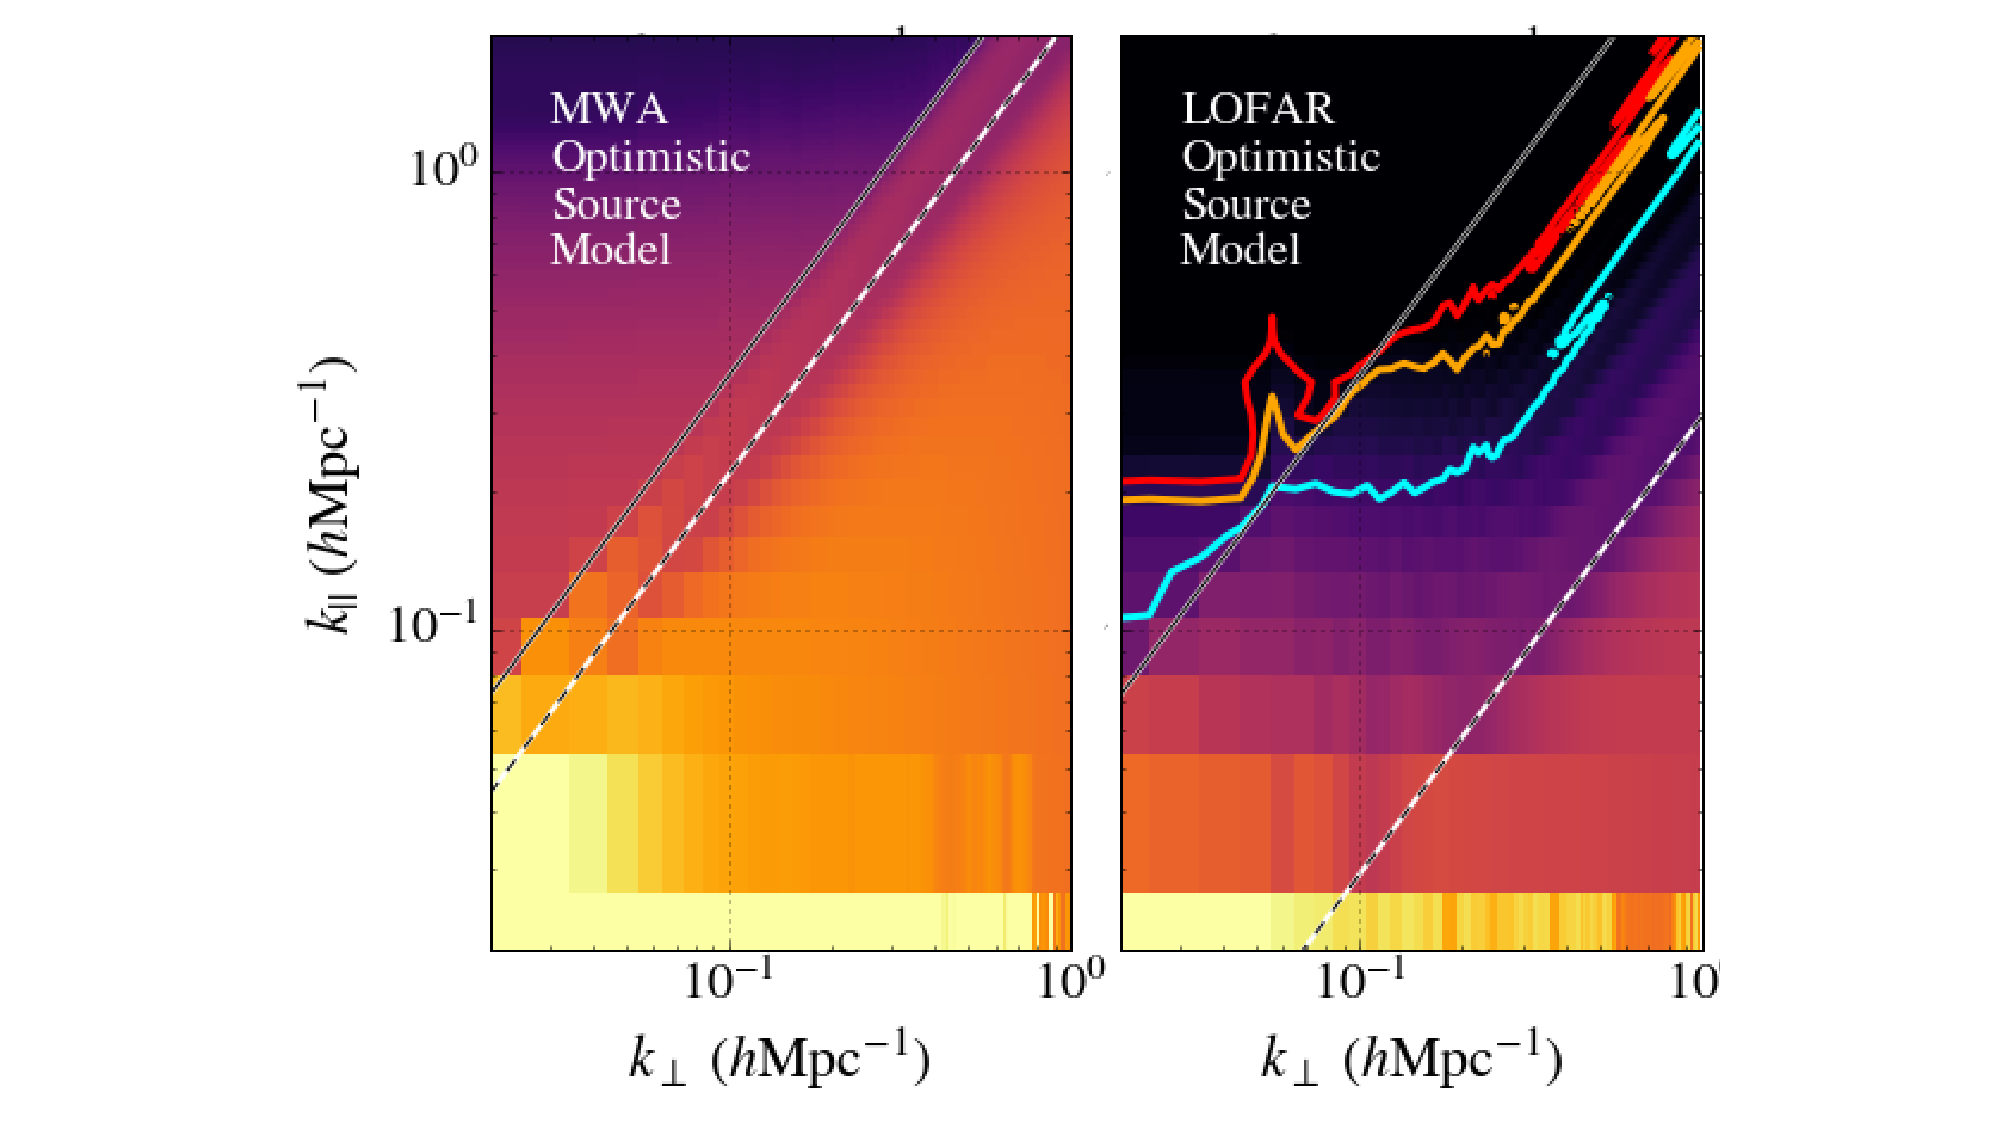
\includegraphics[width=1.\textwidth]{Bernardi/calibration_errors}
\end{center}
\caption{Example of power spectrum bias introduced by calibration errors due to an incomplete sky model for the Murchison Widefield Array (MWA, left) and the Low Frequency Array (LOFAR, right) cases respectively (from \cite{ewall-wice17}). Power spectra are shown in their two dimensional $(k_\perp,k_\parallel)$ form in order to display the foreground dominated region below the horizon limit (grey solid line). Cyan, orange and red lines are the locii where a fiducial 21~cm model power spectrum is one, five and ten times higher than the bias level. In an ideal case with perfectly smooth foregrounds and no calibration errors, the 21~cm power sepctrum should be detectable just outside the horizon limit. The errors introduced by an incomplete sky model leak foreground power in the EoR window at a level that may completely prevent a detection in the MWA case.}
\label{fig:fig_added}
\end{figure}
Sky models are normally constituted of a catalogue of compact sources of known (or measured) properties, often covering an area significantly larger than the telescope field of view (e.g., \cite{yatawatta13}, \cite{pober16}). Nevertheless, sky models remain essentially always incomplete at some level, as source catalogues are limited in depth, source characterization and - often - sky coverage. \cite{grobler14}, \cite{wijnholds16} and \cite{grobler16} show that incomplete catalogues used as sky models bias the calibration and eventually lead to artifacts in the form of ghost-like sources in interferometric images, most of the times fainter than the image noise level. The ghost pattern is stronger for regularly spaced arrays and if the sky model is less complete. In term of power spectrum, \cite{ewall-wice17} and \cite{barry16} show that the calibration bias introduced by incomplete sky models leads to an overall leakage of foreground power in the EoR window (Figure~\ref{fig:fig_added}). A similar foreground leakage may occur because of the finite angular resolution of interferometric observations: for example, two sources whose size is respectively one third and one tenth of the instrument angular resolution will be both modeled as point like even if the first source is only barely unresolved. This biased catalogue would again lead to a leakage of foreground power in the EoR window (\cite{procopio17}). In this case, the bias can be mitigated by obtaining a sky model with an angular resolution much higher than the scales at which the 21~cm signal is expected (\cite{procopio17}).

Sky models that include only compact sources are not adequate for baselines shorter than a few tens of meters as they are sensitive to Galactic diffuse emission, which contributes to most of the power on angular scales $\theta > 10-20$~arcmin (e.g., \cite{bernardi09}, \cite{choudhuri17}). Excluding short baselines from the calibration solutions prevents the problem of modeling diffuse emssion, but can bias the solutions (\cite{patil16}) if the system of calibration equation is not properly regularized (\cite{sardabaradi19}).

In summary, different analsysis approaches provide evidence that {\it imperfect sky models (either because of missing catalogue sources, mis-estimating source properties or missing diffuse emission) are a source of calibration bias that has general effect to corrupt the foreground properties, leaking their power well beyond the ideal horizon limit} and requiring additional modeling and subtraction. For this reason, significant efforts are currently ongoing in order to improve sky models via wider and deeper low frequency surveys (e.g., \cite{hurley-walker17}, \cite{intema17}, \cite{shimwell19}), more accurate low frequency catalogues (\cite{carroll16}) and even better observations of Galactic diffuse emission (\cite{zheng17}, \cite{dowell17}); 
%Some of the calibration strategies described in the next sections may, however, mitigate the requirements of extremely accurate sky models;

\item {\it instrument/primary beam models}. A complete knowledge of a sky model may not be, by itself, sufficient for an accurate calibration of 21~cm observations as the brightness matrix ${\bf B}_I$ is multiplied by the antenna primary beam (equation~ \ref{eq:4} and \ref{eq:sec:3}) and the measurement of an intrinsic sky model requires the separation from the primary beam effect. 

Unlike steerable dishes, most 21~cm interferometers are constituted of dipoles fixed on the ground, in some cases clustered together to form larger stations whose beams that can be digitally pointed to a sky direction by introducing different delays to the dipoles (e.g., like the MWA and LOFAR arrays). As station beams are formed to track the source on the sky, the station projected area changes with time and the shape of the primay beam changes significantly (Figure~\ref{fig:fig3}). This is a typical direction dependent effect that can be casted in the measurement equation as
\begin{equation}
{\bf V}_{12} (u,v,\lambda) = \int_\Omega {\bf E}_1 (t, l, m, \lambda) {\bf B}_{I,s} (l, m, \lambda) \, e^{-2 \pi i (ul + vm)} \, {\bf E}_2^H (t, l, m, \lambda)  dl \, dm,
\label{eq:sec:7_added_2}
\end{equation}
were ${\bf E} (t, l, m, \lambda)$ is the Jones matrix describing the primary beam which, in the simplest cases, is a diagonal matrix:
\begin{equation}
    {\bf E} (t, l, m, \lambda) \equiv 
    \left[
    \begin{array}{cc}
    e_x (t, l, m, \lambda) 	& 	0 	\\
    0 		& e_y (t, l, m, \lambda) 	\\
    \end{array}
    \right].
\label{eq:sec:4}
\end{equation} 
We note that we have written the explicit dependence on the time due to change in projected area for dipole stations and that the direction dependence of the ${\bf E}$ is encoded in its $(l, m)$ dependence.

Time and frequency variable primary beams leads to apparent time variable sky models where variations that are larger away from the pointing direction due to the larger changes in the sidelobe pattern. For examples, sky sources that are well within the main lobe of the primary beam in Figure~\ref{fig:fig3} will experience relatively negligible variations throughout an observation, the opposite will occur to sources located well outside the main lobe as they run through primary beam sidelobes.

Primary beams are also frequency variable and, at first order, their size scales with wavelength (equation~\ref{eq:2}), i.e. rather smoothly. However, in the sidelobe region, variations become rather abrupt as the source can be located on a sidelobe peak at a certain frequency and in the sidelobe null at another frequency. As a final remark, stations that include several dipoles are not perfectly equal to each other, due to manifacturing reasons or mutual coupling between their elements (e.g., \cite{sokolowski17}), therefore ${\bf E}_1 \neq {\bf E}_2$. As primary beams are different, even visibilities for baselines that have the same length and orientation will be different - rather than identical, as expected. The left panel of Figure~\ref{fig:fig3} shows an example of how much primary beams vary for different stations due to mutual coupling interactions: variations in the sidelobe region can be as large as $\sim 30\%$.

If not accurately modeled and taken into account, primary beam effects can bias the calibration solution and, again, corrupt the foreground frequency smoothness.  \cite{bhatnagar08}, \cite{bernardi11}, \cite{sullivan12} and \cite{tasse13} have developed methods to incorporate time and frequency variable primary beams in interferometric images, however, the accuracy of the correction is limited by the accuracy of the primary beam model. Increasing effort is therefore being placed in precise modeling and measurements of the  primary beams (e.g., \cite{pupillo15}, \cite{trott16}, \cite{deleraacedo17}, \cite{trott17a}, \cite{jacobs17}, \cite{deleraacedo18});
\begin{figure}[]
\begin{center}
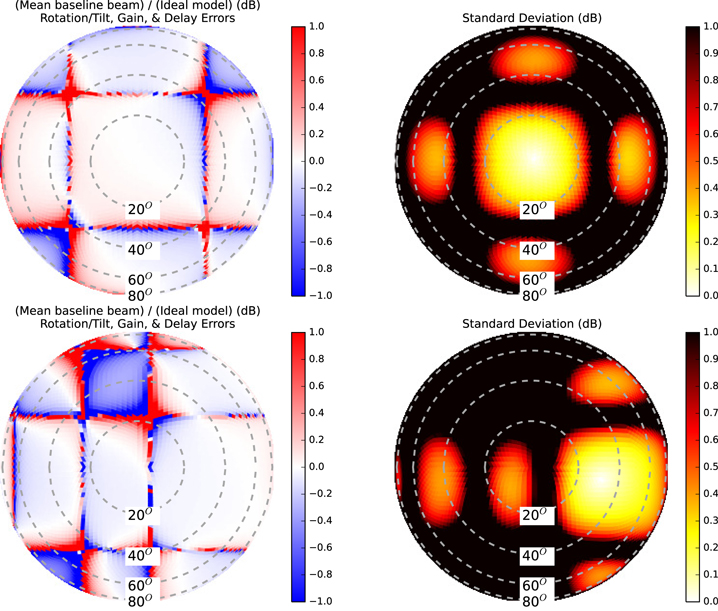
\includegraphics[width=1.\textwidth]{Bernardi/mwa_beams_err}
\end{center}
\caption{Example of primary beam variations as the MWA station points at zenith (top right) and $\sim 30^\circ$ away from zenith (bottom right) at 150~MHz. The left column shows the fractional variation of individual station beam models, with respect to the nominal primary beam (right column, from \cite{neben16}. It is visibile how different the sidelobe pattern is when pointing towards two different directions. It should also be noticed the $\sim 10\%$ magnitude of the first lobe and the large null regions around the sidelobes. The specific pattern is due to the regular shape of the MWA station, where 16 dipoles are arrange in a square $4 \times 4$ grid.}
\label{fig:fig3}
\end{figure}


\item {\it polarization leakage calibration}. Equation~\ref{eq:sec:3} and \ref{eq:sec:7} show that, even if the 21~cm signal is unpolarized, care needs to be taken against the contamination from polarized foreground emission. Most point sources are unpolarized below 200~MHz (\cite{bernardi13}, \cite{lenc16}, \cite{vaneck18}), therefore the assumption of an unpolarized sky model is well justified. However, calibration errors (in the matrix ${\bf B}$) would lead  to a relative miscalibration of the $xx$ and $yy$ polarizations and, in turn, to leakage of polarized emission into total intensity. This effect may be particularly strong on short baselines (e.g., shorter than a $\sim 1$~km), where polarized foregrounds are brighter (\cite{bernardi09}, \cite{iacobelli13}, \cite{jelic15}, \cite{lenc16}). Polarized foregrounds that are Faraday rotated by the interstellar medium and leak to total intensity are a severe contamination to the 21~cm signal: they have a characteristic frequency dependence similar to the 21~cm signal therefore have power across the whole EoR window and cannot be subtracted using standard methods (e.g., \cite{jelic10}, \cite{moore13}, \cite{nunhokee17}).  

Even if calibration errors are negligible, low frequency antennas have a non negligible polarized response across their wide field of view, i.e. the primary beam Jones matrix ${\bf E}$ is no longer diagonal. The measurement equation with a full polarized primary beam response can be written as (\cite{nunhokee17}):
\begin{eqnarray}
    \left[ 
    \begin{array}{cc}
    V_{12,I} (u,v,\lambda)\\
    V_{12,Q} (u,v,\lambda)\\
    V_{12,U} (u,v,\lambda)\\
    V_{12,V} (u,v,\lambda)
    \end{array}
    \right] & = & \int_\Omega{ {\bf S}^{-1} [ {\bf E}_1 \otimes {\bf E}_2^H ] {\bf S} 
    \left[ 
    \begin{array}{cc}
    I (l,m,\lambda)\\
    Q (l,m,\lambda)\\
    U (l,m,\lambda)\\
    V (l,m,\lambda)
    \end{array}
    \right]
     \, e^{-2 \pi i (ul + vm)} dl \, dm } = \nonumber \\
     & = & \int_\Omega{ {\bf A} (l,m,\lambda) 
    \left[ 
    \begin{array}{cc}
    I (l,m,\lambda)\\
    Q (l,m,\lambda)\\
    U (l,m,\lambda)\\
    V (l,m,\lambda)
    \end{array}
    \right]
     \, e^{-2 \pi i (ul + vm)} dl \, dm },
\label{eq:sec:8}
\end{eqnarray} 
where ${\bf S}$ is the matrix that relates the intrisic Stokes parameters to the observer $x-y$ frame (\cite{hamaker96}) and $\otimes$ is the outer product. Visibilities are written as a four-element vector as this form shows that the ${\bf A}$ matrix maps the intrinsic Stokes parameters into the observed ones: 
\begin{eqnarray}
    \left(
    \begin{array}{cccc}
    I' \leftarrow I & I' \leftarrow Q & I' \leftarrow U & I' \leftarrow V \\
    Q' \leftarrow I & Q' \leftarrow Q & Q' \leftarrow U & Q' \leftarrow V \\
    U' \leftarrow I & U' \leftarrow Q & U' \leftarrow U & U' \leftarrow V \\
    V' \leftarrow I & V' \leftarrow Q & V' \leftarrow U & V' \leftarrow V \\
    \end{array}
    \right).
\label{eq:sec:9}
\end{eqnarray} 
An example of ${\bf A}$ matrix is shown in Figure~\ref{fig:fig4}. The first raw of the matrix shows how the four intrisinc Stokes parameters contribute to the observed total intensity and, therefore, how polarized foregrounds leak into the 21~cm signal even in absence of any calibration errors: the magnitude of the contaminating Stokes $Q$ and $U$ foregrounds increases away from the ponting direction. Wide-field polarization is another textbook example of direction dependent calibration problem.

Calibration of polarization leakage remains a challenging task. Instruments with marrow fields of view naturally mitigate the leakege (\cite{asad15}, \cite{asad16}, \cite{asad18}). It can also be mitigated by extending the sky model to include polarization (e.g. \cite{geil11}), although modeling the diffuse Galactic foreground - the brightest component - is not straightforward and requires accurate imaging. However, \cite{nunhokee17} show that the magnitude of the Galactic polarization leakage may be below the 21~cm signal at high $k_\parallel$ values ($k_\parallel > 0.3$~Mpc$^{-1}$) and, therefore, still be ``avoided". A more extensive characterization of the polarized foreground properties is needed in order to extend their results to a general case.
\begin{figure}[]
\begin{center}
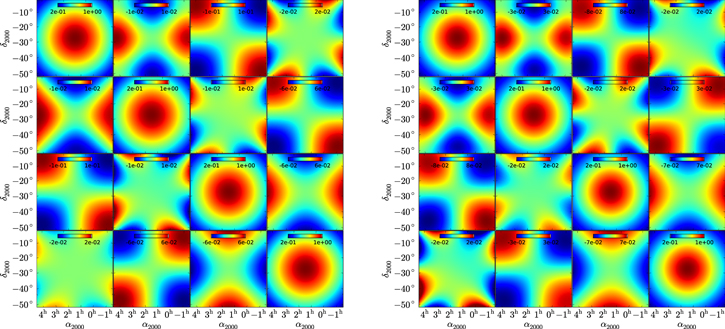
\includegraphics[width=1.\textwidth]{Bernardi/polarized_beam_leakage}
\end{center}
\caption{Examples of ${\bf A}$ matrices at 130 (left) and 150~MHz respectively (from \cite{nunhokee17}). The matrix maps the intrinsic Stokes parameters into observed ones: the diagonal terms represent the standard primary beam patterns, whereas the off-diagonal terms are the leakage terms. The second, the third and the fourth element of the first row show how Stokes parameters $Q$, $U$ and $V$ respectively contaminate the total intensity signal.}
\label{fig:fig4}
\end{figure}



\begin{figure}[]
\begin{center}
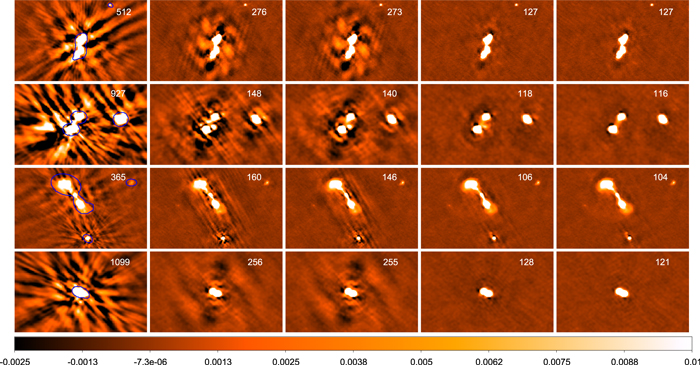
\includegraphics[width=1.\textwidth]{Bernardi/ionospheric_calibration}
\end{center}
\caption{Calibration of ionospheric effects in LOFAR observations using a faceting algorithm (from \cite{vanweeren16}). The image resolution is $8'' \times 6''.5$ and the $120-180$~MHz bandwidth is used. The left column shows zoom in images around sources without direction dependent calibration which is, in turn, applied incrementally towards the right panels. For each of the sources, a sky model and a direction dependent Jones scalar $Z$ is improved at each iteration until an artefact-free image is obtained (right column). Solutions were computed each 10~s. An additional amplitude calibration to account for primary beam variations was determined on scales of 10~minutes. The colour scale is in units of Jy~beam$^{-1}$.}
\label{fig:fig5}
\end{figure}
\item {\it ionospheric distortions}. The ionosphere is the partially ionized layer situated between $\sim 50$ and 1000~km above the surface of the Earth, whose electron density changes with time and position. At low frequencies the ionosphere is no longer transparent to radio waves and, to first order, it introduces a delay $\phi$ in the wave propagation proportional to the integral of the electron density along the line of sight (e.g. \cite{TMS}, \cite{intema09}):  
\begin{equation}
\phi (t, \nu) \propto \frac{1}{\nu} \int n_e (t) dl;
\label{eq:sec:11}
\end{equation}
where the integral is the total electron content (TEC). When the delay is different for two different antennas, vibilities measure an additional, time variable delay. In the measurement equation formalism, ionospheric delays can be modeled by a scalar term $Z \propto e^{i\phi (t,\nu)}$, however, ionospheric effects are another texbook example of direction dependent calibration as the $Z$ is often different for different directions. Given the size $S$ of a characteristic ionospheric patch where the TEC is constant, direction dependent effects occur when the field of view is much larger than $S$ or the baseline separation is much larger than $S$, i.e. different antennas ``see through" different TEC values (see \cite{intema09} for extensive discussion on the different ionospheric regimes). In this case, the measurement equation takes a form similar to equation~\ref{eq:sec:7_added}: 
\begin{equation}
{\bf V}_{12} (u,v,t,\lambda) = \sum_s Z_{1,s} (t, \lambda) \left ( \int_\Omega {\bf B}_{I,s} (l, m, \lambda) \, e^{-2 \pi i (ul + vm)} \,  dl \, dm \right ) Z_{2,s}^H (t, \lambda),
\label{eq:sec:12}
\end{equation}
leading to images where sources are convolved with a position and time dependent PSF. An example of this effect is shown in Figure~\ref{fig:fig5}: the column on the left shows sources after the standard selfcalibration, still surrounded by artifacts due to the ionosphere; moving towards the right,  iterative direction dependent corrections lead to virtually artefact-free images on the right column (see \cite{vanweeren16} for further details). 

\cite{trott17b} analyzed the effects of ionospheric perturbations on MWA observations, whose maximum baseline is a factor of $\sim 30$ shorter than the LOFAR example displayed in Figure~\ref{fig:fig5}, but with a field of view $\sim 4$ times larger. They found that direction dependent ionospheric distortions can affect the sky coherence up to degree-scales (i.e. scales relevant for 21~cm observations), however, due to the relatively short baselines, these effects occur only in 8\% of the observations and it is relatively straightforward to monitor the ionospheric activity and exclude the most affected observations.

An extensive modeling of the impact of ionospheric errors on the two dimensional $(k_\perp,k_\parallel)$ power spectrum spectrum has been carried out by \cite{vedantham16}. They found that most of the residual effects due to the ionosphere on baselines shorter than a few km are confined within the horizon limit, therefore not impacting foreground avoidance. Moreover, the frequency coherence of the ionospheric residuals is such that they will likely be removed by foreground subtraction algorithm.

Current investigations seem therfore to suggest that ionospheric effects are not going to be a show stopper for 21~cm power spectrum observations and, likely, 21~cm tomography. 
\end{itemize}





\subsection{Redundant calibration}

An interferometric array where most of the baselines have the same length and orientation is called {\it redundant} as they measure the same Fourier mode of the sky brightness distribution. Redundant array configurations are often not appealing as they have poor imaging performances because they do not measure sufficient Fourier modes to reconstruct accurate sky images. However, a maximally redundant array where the antennas are laid out in a regularly spaced square grid offers the maximum power spectrum sensitivity on the $k_\perp$ modes corresponding to the most numerous baselines. This criterium has inspired the highly redundant layouts of the MIT Epoch of Reionization experiment (\cite{zheng14}), the Precision Array to Probe the Epoch of Reionization (PAPER, \cite{parsons12b}) and partly driven the updated MWA.

One of the advantages of a redundant array is that it enables a different calibration strategy called {\it redundant calibration}. In redundant calibration the form of the measurement equation does not change and can be written, for a single polarization, like equation~\ref{eq:sec:7}:
\begin{equation}
V_{12,xx} (u,v,\lambda) = b_{1,x} \, b_{2,x}^* y_{12,xx} (u,v,\lambda),
\label{eq:sec:13}
\end{equation}
with the difference now that the model visibility $y$ is not tied to a sky model, but it is solved for, simply assuming that it is the same for each group of redundant baselines {\cite{wieringa92}, \cite{liu10}). In other words, redundant calibration is independent on the sky model and, therefore, bypasses entirely the biases related to sky model incompleteness described in Section~\ref{sec:challenges}. However, as redundant calibration is not tied to any physical (i.e. sky-based) spatial or spectral model, its solutions have degeneracies that need to be solved for by using a sky model (e.g., \cite{zheng14}, \cite{byrne19}). In particular, spectral calibration, which is critical for foreground separation, cannot currently be obtained using redundant calibration and requires a sky-based calibration. \cite{byrne19} suggest that sky model incompleteness can bias this calibration step, in a way similar to what happens with a traditional calibration scheme. Moreover, as redundant calibration is agnostic of the polarization state of the sky brightness distribution, mitigation of polarization leakage remains an open question in the framework of redundant calibration (\cite{dillon18}). 

Finally, redundant calibration is prone to effects that break the assumption of redundancy, the most common being errors in the antenna positions and different primary beams for different antennas. Antenna position errors can be reduced to have a negligible impact on redundant calibration \cite{joseph18}. The effect of primary beam variations amongst the different antennas on redundant calibration is likely more severe, although new calibration schemes seem to be able to mitigate it (\cite{orosz19}).



\section{Array design and observing strategies}
\label{sec:design}

\begin{figure}[]
\begin{center}
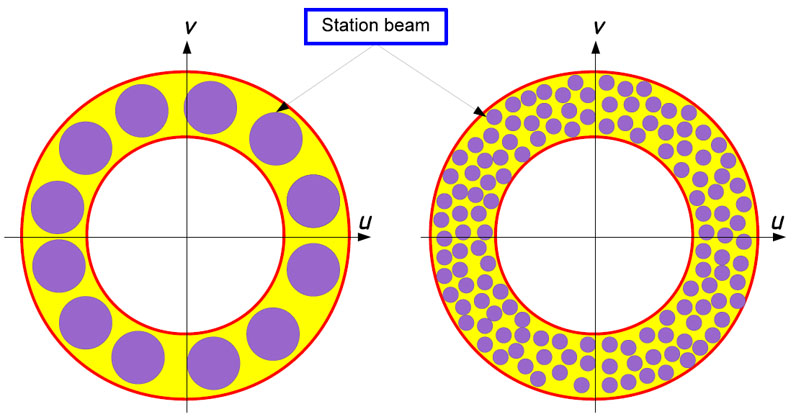
\includegraphics[width=1.\textwidth]{Bernardi/uv_footprint}
\end{center}
\caption{Cartoon illustration of the $uv$ footprint due to the primary beam (from https://ned.ipac.caltech.edu/level5/March14/Zaroubi/Zaroubi5.html\#5.1). The purple circles are the $uv$ footprints for a large (right panel) and small (left panel) station respectively. The minimum and maximum baselines is the same for both cases, in order to sample the same $uv$ annulus (yellow area).}
\label{fig:fig6}
\end{figure}
I will conclude this chapter by discussing how the various interferometric effects discussed so far impact the choice of array designs and the consequent observing strategies. \cite{morales05} and \cite{parsons12b}, for example, investigate how instrumental choices like the array layout, the antenna size and the bandwidth (do not) affect the 21~cm power spectrum spectrum. Here I would rather emphasize on the interdependence between instrumental choices, calibration and foreground separation strategies. If the total collecting area is kept fixed, there are two main elements that impact calibration and foreground separation strategies:
\begin{itemize}
\item {\it station size}. The choice of the station size determines the minimum $k_\perp$ value accessible and the footprint of each $uv$ measurement. Each visibility is not a single point in the $uv$ plane but has a footprint corresponding to the two dimensional Fourier transform of the primary beam. This can be seen using the convolution theorem to re-write equation~\ref{eq:1}: \begin{equation}
V_{ij} ({\bf b}, \lambda) = \tilde{A} ({\bf b}, \lambda) \ast \tilde{I} ({\bf b}, \lambda).
\end{equation}
Smaller stations have smaller footprints in the $uv$ plane (see Figure~\ref{fig:fig6}) and can, therefore, sample the $uv$ more accurately with respect to larger stations. They also allow to probe smaller $k_\perp$ values (as the minimum possible $uv$ length is essentially the station size) for which the avoidance strategy is more effective (see Figure~\ref{fig:fig2}).
If smaller stations would be preferred for power spectrum measurements, they are generally more challenging in terms of calibration: their wider fields of view require a more accurate sky model for calibration, are more susceptible to ionospheric effects and suffer from a more severe polarization leakge contamination. Given the smaller size, their visibilities have a lower signal-to-noise ratio compared to larger station that can lead to limitations to the calibration of high time variable effects. On the other hand, they do not necessarily require to track sources with a high time cadence but can use drift scan strategies (where they are pointed to a fied direction and the sky drifts overhead) or a mix of drift scan and pointed observations to maximize sensitivity (\cite{trott14}). The advantage of drift scan over pointed observations is that primary beams remain constant in time, avoiding some of the effects described in the Section~\ref{sec:challenges}.

\item {\it array layout}. Beyond the obvious sensitivity requirement that prefers compact arrays due to their better brightness sensitivity, layout choices are also intrinsically related to calibration and foreground separation strategies. A pseudo-random station distribution that leads to a filled $uv$-coverage (between the minimum and the maximum station separation) is highly desirable for imaging, modeling and subtracting foregrounds. It is not a stringent requirement for power spectrum measurement and for the avoidance strategy. It is probably necessary for 21~cm tomography, in order to provide recostrunction of the low-brightness neutral Hydrogen regions.

On the opposite side of the spectrum of choices, redundant arrays are the most sensitive power spectrum machines. They obviously leverage on redundant calibration which is precluded to imaging arrays. Their drawbacks are the poor imaging performances that prevent the accurate foreground modeling and essentially only allow foreground avoidance. For the same reason, if redundant calibration is not sufficient, redundant arrays have limited options to improve calibration by recostructing the sky brightness sensitivity.   
\end{itemize}

I will use four existing low frequency arrays as examples of the range of cases of interest:
\begin{itemize}
%\item effect of the field of view, calibratability, uv cell, drift scan versus tracking, suppression of sources outside the main lobe ionosphere
%\item uv coverage choices power spectra vs images, redundant vs pseud random (reconstructing sky brightness), minimum/maximum k mode accessible... avoidance (compact) vs subtraction (less compact)
%\item obviously sensitivity

\item {\it Low Frequency Array (LOFAR, \cite{vanhaarlem13})}. LOFAR is an array of 40 stations located in The Nerthelands and several remote stations across Europe. 24 stations are located in a 2~km core from the array centre and the remaining stations are distributed in a logarithmic spiral layout up to $\sim 100$~km, providing a very dense $uv$ coverage in a few hours tracked observation (see Chapter~8 in this book for an image of the LOFAR array layout and the other arrays discussed in this Section).

Stations are formed by two types of receptors sensitive to the $30-90$ and $110-200$~MHz respectively. The $110-200$~MHz stations are the most sensitive to 21~cm observations and we will only consider them in this discussion. They are constituted by 48 clusters of dipoles (each of them being a $4 \times 4$ square grid) arranged in a regular $\sim 30$~m diameter grid, leading a $\sim 4^\circ$ field of view at 150~MHz.

LOFAR is an example of a traditional interferometric array, with excellent point source sensitivity that favours the sky-based calibration and very dense $uv$ coverage for high fidelity imaging. Its large station size has a large $uv$ footprint but also a relatively narrow field of view that essentially requires tracking a sky patch. The narrow field of view allows to select sky patches with low foreground (including polarization) contamination and to reject wide field foreground emission. Unwanted sky emssion far from the pointing direction is further suppressed by rotating each station grid with respect to another, while rotating the dipoles back to a common polarization frame: this operation makes the station primary beams all different and the different sidelobe patterns, that would otherwise be reinforced by the regular station grid, cancel out each others.

The calibration of LOFAR 21~cm observations relies on an accurate sky model where compact sources are modeled using the longest baselines available (i.e. $\sim 100$~km). Direction dependent calibration corrects ionospheric effects that corrupt visibilities on baselines longer than a few km, and the effect of variable primary beams on compact sources (\cite{yatawatta13}). The sky model is then subtracted from the visibilities and residual foregrounds are subtracted in the image domain (see details in Chapter~6 in this book). 

The LOFAR design is suited for 21~cm tomography on large angular scales, providing foregrounds are adequately subtracted (\cite{zaroubi12}).

\item {\it Murchison Widefield Array (MWA, \cite{tingay13}, \cite{wayth18})}. The MWA is an array located in Western Australia, operating between 80 and $\sim 200$~MHz. It employs the same LOFAR dipoles, although they are assembled in stations of $4 \times 4$ elements arranged in a regular grid. The station size is therefore $\sim 6$ times smaller compared to LOFAR, with an equivalent increase of the field of view. 
The MWA underwent a recent upgrade to phase II (to distinguish it from the initial deployment, named phase I) and is now constituted of 256 stations (out of which only 128 can be simultaneously correlated) in a hybrid configuration: 128 stations are deployed in a pseudo random configuration out to a $\sim 3$~km baseline (the phase I telescope), 72 stations in two highly redundant hexagons next to the core of the array and 56 stations to extend the maximum baseline up $\sim 5$~km. 

MWA phase II is a fairly versatile instrument: in its compact, redundant configuration, it is optimized for power spectrum observations and can leverage redundant calibration (\cite{li18}); its small stations give a good sampling in the $uv$ plane (right panel case in Figure~\ref{fig:fig6}). In its extended configuration it has an exceptionally good instantaneous $uv$ coverage (due to the high number of stations instantaneously correlated) with low sidelobe levels, which is good for imaging and foreground modeling, and a large field of view which allows to survey the sky very quickly. The wide field of view does not allow to isolate low foreground patches, but it allows to opt for drift scan observations or a mix of drift scan and pointed observations (\cite{trott14}), which have the advantage of more time stable primary beams. Wide field ionospheric effects are somewhat mitigated by the array compactness (\cite{jordan17}).
The MWA can therefore leverage on the strength of both redundant and traditional calibration and can adopt a mixture of foreground subtraction and avoidance strategies.

The MWA approach has, however, limitations too: the regular station grid (without any rotation, unlike LOFAR) generates strong sidelobes (see Figure~\ref{fig:fig3}) which make calibration and foreground separation more challenging; the large field of view requires more comprehensive sky models fore calibration and is more susceptible to polarization leakage; the relatively short maximum baseline may be insufficient to derive accurate sky models (\cite{procopio17}). 

\item {\it Precision Array to Probe the Epoch of Reionization (PAPER, \cite{parsons10})}. PAPER was an array located in the South Africa, operating in the $100-200$~MHz range and now decommissioned in favour of its successor (the Hydrogen Epoch of Reionization Array, see Chapter~\ref{chapter:koopmans_bernardi} in this book). It employed custom designed $\sim 2$~m dipoles that were deployed and re-arranged in several configurations up to a 128~element array. Dipoles were always individually correlated with no clustering into larger stations, implying a nearly all-sky field of view instrument. In order to maximize power spectrum sensitivity, dipoles were always deployed in maximally redundant configuration with very short baselines (up to a maximum of 350~m), enabling the advantages of redundant calibration (\cite{parsons14}, \cite{ali15}, \cite{jacobs15}). In the final 128-element deployment, $\sim 20$ dipoles were placed as outriggers out of the regular grid in order to partially improve the $uv$ coverage for foreground characterization and calibration. 

In some sense, PAPER represents the choice opposite to the LOFAR case: an almost fully redundant array that works using essentially only foreground avoidance and without any spatial characterization of foregrounds for either calibration or subtraction. PAPER is a full drift scan array with primary beams that are fairly stable with time, but also with an all-sky field of view where no selection of low foreground regions is possible, for which polarization leakage and ionospheric effects are more severe, although the latter are mitigated by the very compact configuration. 

As pointed out earlier in this chapter, a redundat array like PAPER is not suited for 21~cm tomography.
\end{itemize}


\section{Conclusions}
\label{sec:conclusions}

This chapter presented a summary of interferometry and calibration in the light of 21~cm observations. I started from the basics of interferometry to show how they are related to observations of the 21~cm power spectrum and its tomographic images. I reviewed calibration of 21~cm observations, highlighting how foreground separation - the biggest challenge of 21~cm observations - critically depends various calibration effects (sky models, primary beam modeling and calibration, polarization leakage, the ionosphere). I also attempted to show how the various array designs adopted by current experiments enable different calibration and observational strategies - neither of which is clearly winning, at the present point. The field is rapidly developing and both current and upcoming instruments (see Chapter~\ref{chapter:koopmans_bernardi} in this book) will address some of the open questions presented in this chapter.






%Lorem ipsum dolor sit amet, consectetur adipiscing elit. Duis eu egestas erat. Maecenas tincidunt lacinia tincidunt. Mauris id lectus nec neque feugiat condimentum vitae at diam. In vel orci nunc, non commodo mauris. Vivamus ipsum enim, vulputate quis pharetra non, molestie quis felis. Vivamus porttitor placerat turpis at accumsan. Nunc tortor velit, faucibus a rhoncus nec, blandit non elit. Nam consectetur lectus eu nisi blandit dapibus rhoncus dui tempus. Mauris fermentum dolor vel ipsum vulputate sit amet ultricies tortor lacinia. Donec ut nibh erat. Morbi nec mi ante. Integer nec vestibulum diam. Donec tincidunt pellentesque quam, ut interdum mauris venenatis condimentum. Nam condimentum, augue in aliquet gravida, neque dui elementum eros, id semper eros purus sed felis. Curabitur in justo sit amet sapien ultrices hendrerit at quis nibh. Quisque iaculis pulvinar tincidunt. 
%\begin{eqnarray}
%C(12) &= &\left[\overrightarrow{\pi}\cdot\overrightarrow{\phi}(x+r)\right] \nonumber \\ 
%&\approx& 1-\mathrm{const}\frac{r^2}{L^2}\int_r^L\frac{x\rmd x}{x^2} + \cdots \nonumber  \\
%&\approx& 1-\mathrm{const}\frac{r^2}{L^2}\ln\frac{x\rmd x}{x^2} + \cdots .\label{brokenlongeqn}
%\end{eqnarray}
%
%Aenean tellus risus, porta sit amet porta vitae, tincidunt ut felis. Class aptent taciti sociosqu ad litora torquent per conubia nostra, per inceptos himenaeos. Vestibulum ante ipsum primis in faucibus orci luctus et ultrices posuere cubilia Curae; Phasellus pulvinar placerat velit auctor egestas. Vivamus euismod fringilla tincidunt. Sed ut magna felis, id sollicitudin nunc. Quisque a dui eu erat consectetur egestas a quis justo. Aenean euismod congue diam, vel posuere urna fermentum sit amet. Lorem ipsum dolor sit amet, consectetur adipiscing elit. Mauris faucibus lacus eget est mollis auctor. Donec at nibh ligula, et posuere massa. Phasellus quis leo diam \cite{diamantaras1996pcn}.
%Donec aliquam blandit risus, eu venenatis ante euismod eu. Curabitur cursus justo id arcu condimentum feugiat. Integer sapien urna, vulputate et adipiscing nec, convallis et justo. Suspendisse in ipsum at felis ornare interdum \cite{tulone2006pts},
%
%\begin{figure}[]
%\begin{center}
%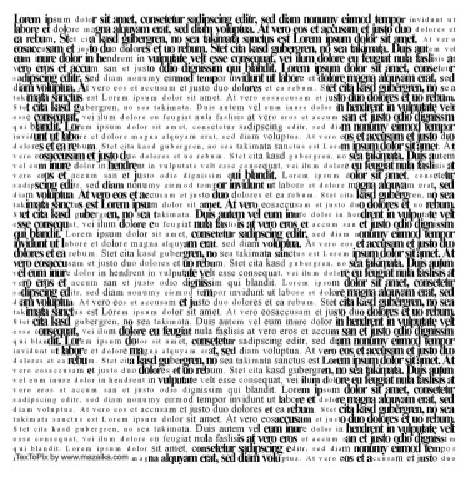
\includegraphics[width=0.5\textwidth]{Bernardi/01x01-eps-converted-to}
%\end{center}
%\caption{This is figure 1 in chapter 1.}
%\end{figure}
%
%\paragraph{Cras adipiscing} sagittis nunc vel luctus. Suspendisse volutpat augue quis erat semper consequat dignissim tellus euismod. Morbi hendrerit, tellus id aliquam iaculis, nibh leo tincidunt eros, vitae varius ligula felis in mi.
%
%\begin{table}
%\caption{Greek Letters.}
%\begin{center}
%\begin{tabular}{llllllll}
%\hline
%$\alpha $  & $ \beta $  & $ \gamma $  & $ \delta $  & $ \epsilon $  & $ \varepsilon $  & $ \zeta $  & $ \eta $ \\
% $ \theta $  &  $ \vartheta $  &  $ \gamma $  &  $ \kappa $  &  $ \lambda $  &  $ \mu $  &  $ \nu $  &  $ \xi $ \\
% $ o $  &  $ \pi $  &  $ \varpi $  &  $ \rho $  &  $ \varrho $  &  $ \sigma $  &  $ \varsigma $  &  $$ \\
% $ \tau $  &  $ \upsilon $  &  $ \phi$ &  $ \varphi $  &  $ \chi $  &  $ \psi $  &  $ \omega$  &  $ $ \\
% &  &  &  &  &  &  & \\
%$ \Gamma $  & $ \Delta $  & $ \Theta $  &  $ \Lambda $  &  $ \Xi $  &  $ \Pi $  &  $ \Sigma $  & $ \Upsilon $ \\
% $ \Phi$ &  $ \Psi $  &  $ \Omega $  &  &  &  &  &\\
%\hline
%\end{tabular}
%\end{center}\end{table}
%
%\begin{figure}[]
%\begin{center}
%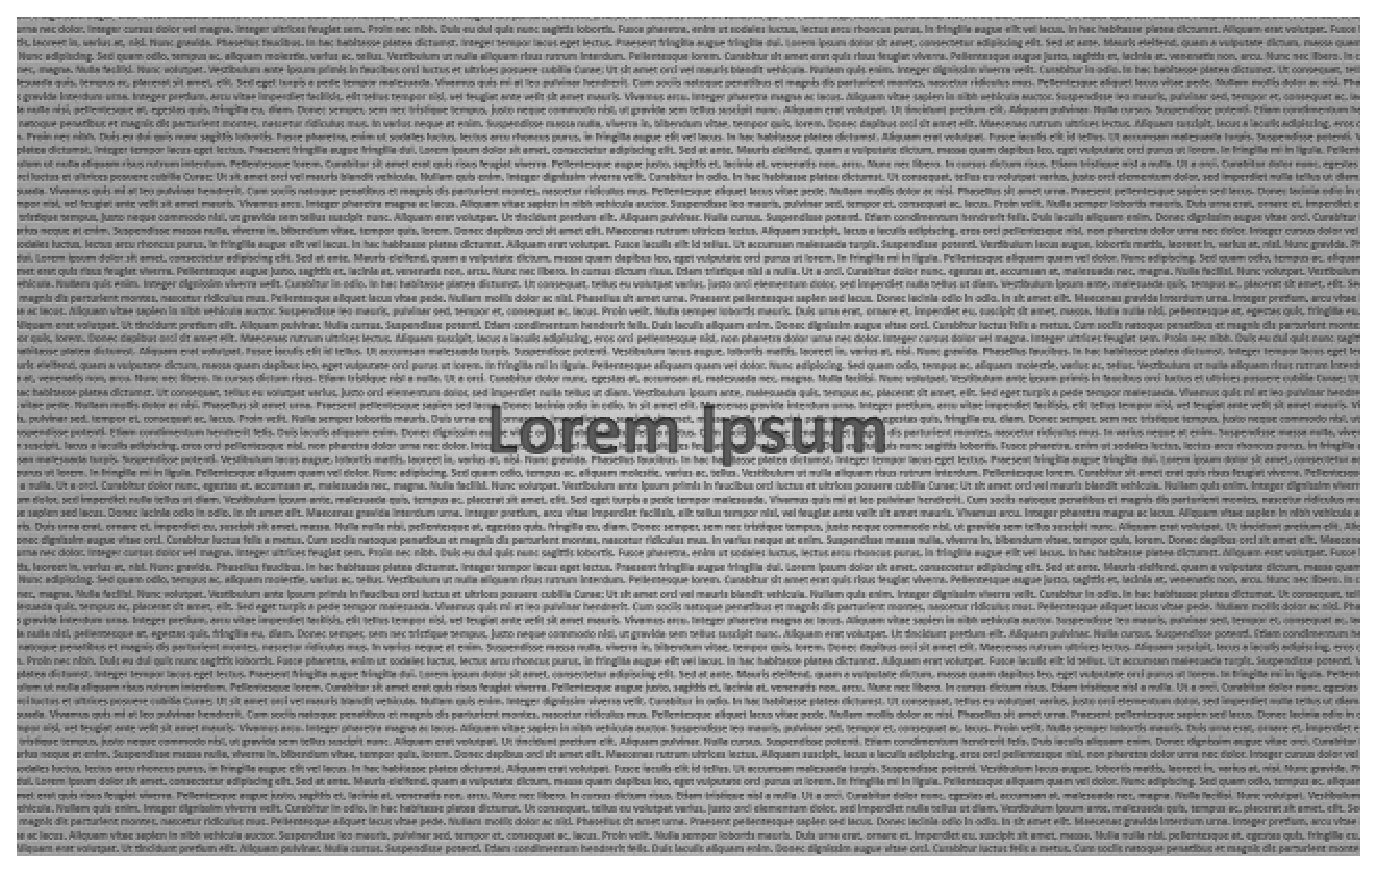
\includegraphics[width=0.6\textwidth]{Bernardi/01x02}
%\end{center}
%\caption{This is figure 2 in chapter 1.}
%\end{figure}
%
%
\bibliographystyle{plain}
\bibliography{Bernardi/References}


